\chapter{Softwarekonzept} \label{chap:Konzept}

Der dieser Studienarbeit zu Grunde liegende Code wurde in der letzten Studienarbeit in einer Cloud-Umgebung entwickelt. Als einfache testumgebung zur umsetzung einer Machbarkeitsstudie war dies ausreichend. 
Da in dieser Studienarbeit das Umsetzen einer Webvisualisierung der durch die FESTO \ac{cp-lab} aufgenommenen Daten im Vordergrund steht, ist es notwendig, die Software in eine lokale Umgebung zu verschieben. 
Dies ermöglicht eine bessere Kontrolle über die Entwicklungsumgebung und die verwendeten Bibliotheken. 

Zusätzlich sollen alle einstellbaren Parameter zentral aufgeführt werden. Dies ermöglicht eine einfache Konfiguration der Software und entspricht dem Stand der Technik\cite{gur_diskussion_2024} \cite{oliveira_how_2023}. 

Die Realisierung beider Aufgaben wird in diesem Kapitel beschrieben

\section{Programmstruktur} \label{sec:architektur}

Erster Teil der Softwarekonzeption ist der Entwurf der Struktur. Die Struktur einer Software ist entscheidend für die Wartbarkeit und Erweiterbarkeit. Zwei wichtige Kriterien, deren Erhaltung im gesamten Designprozess berücksichtigt werden muss.

\begin{figure}[H]
    \centering
    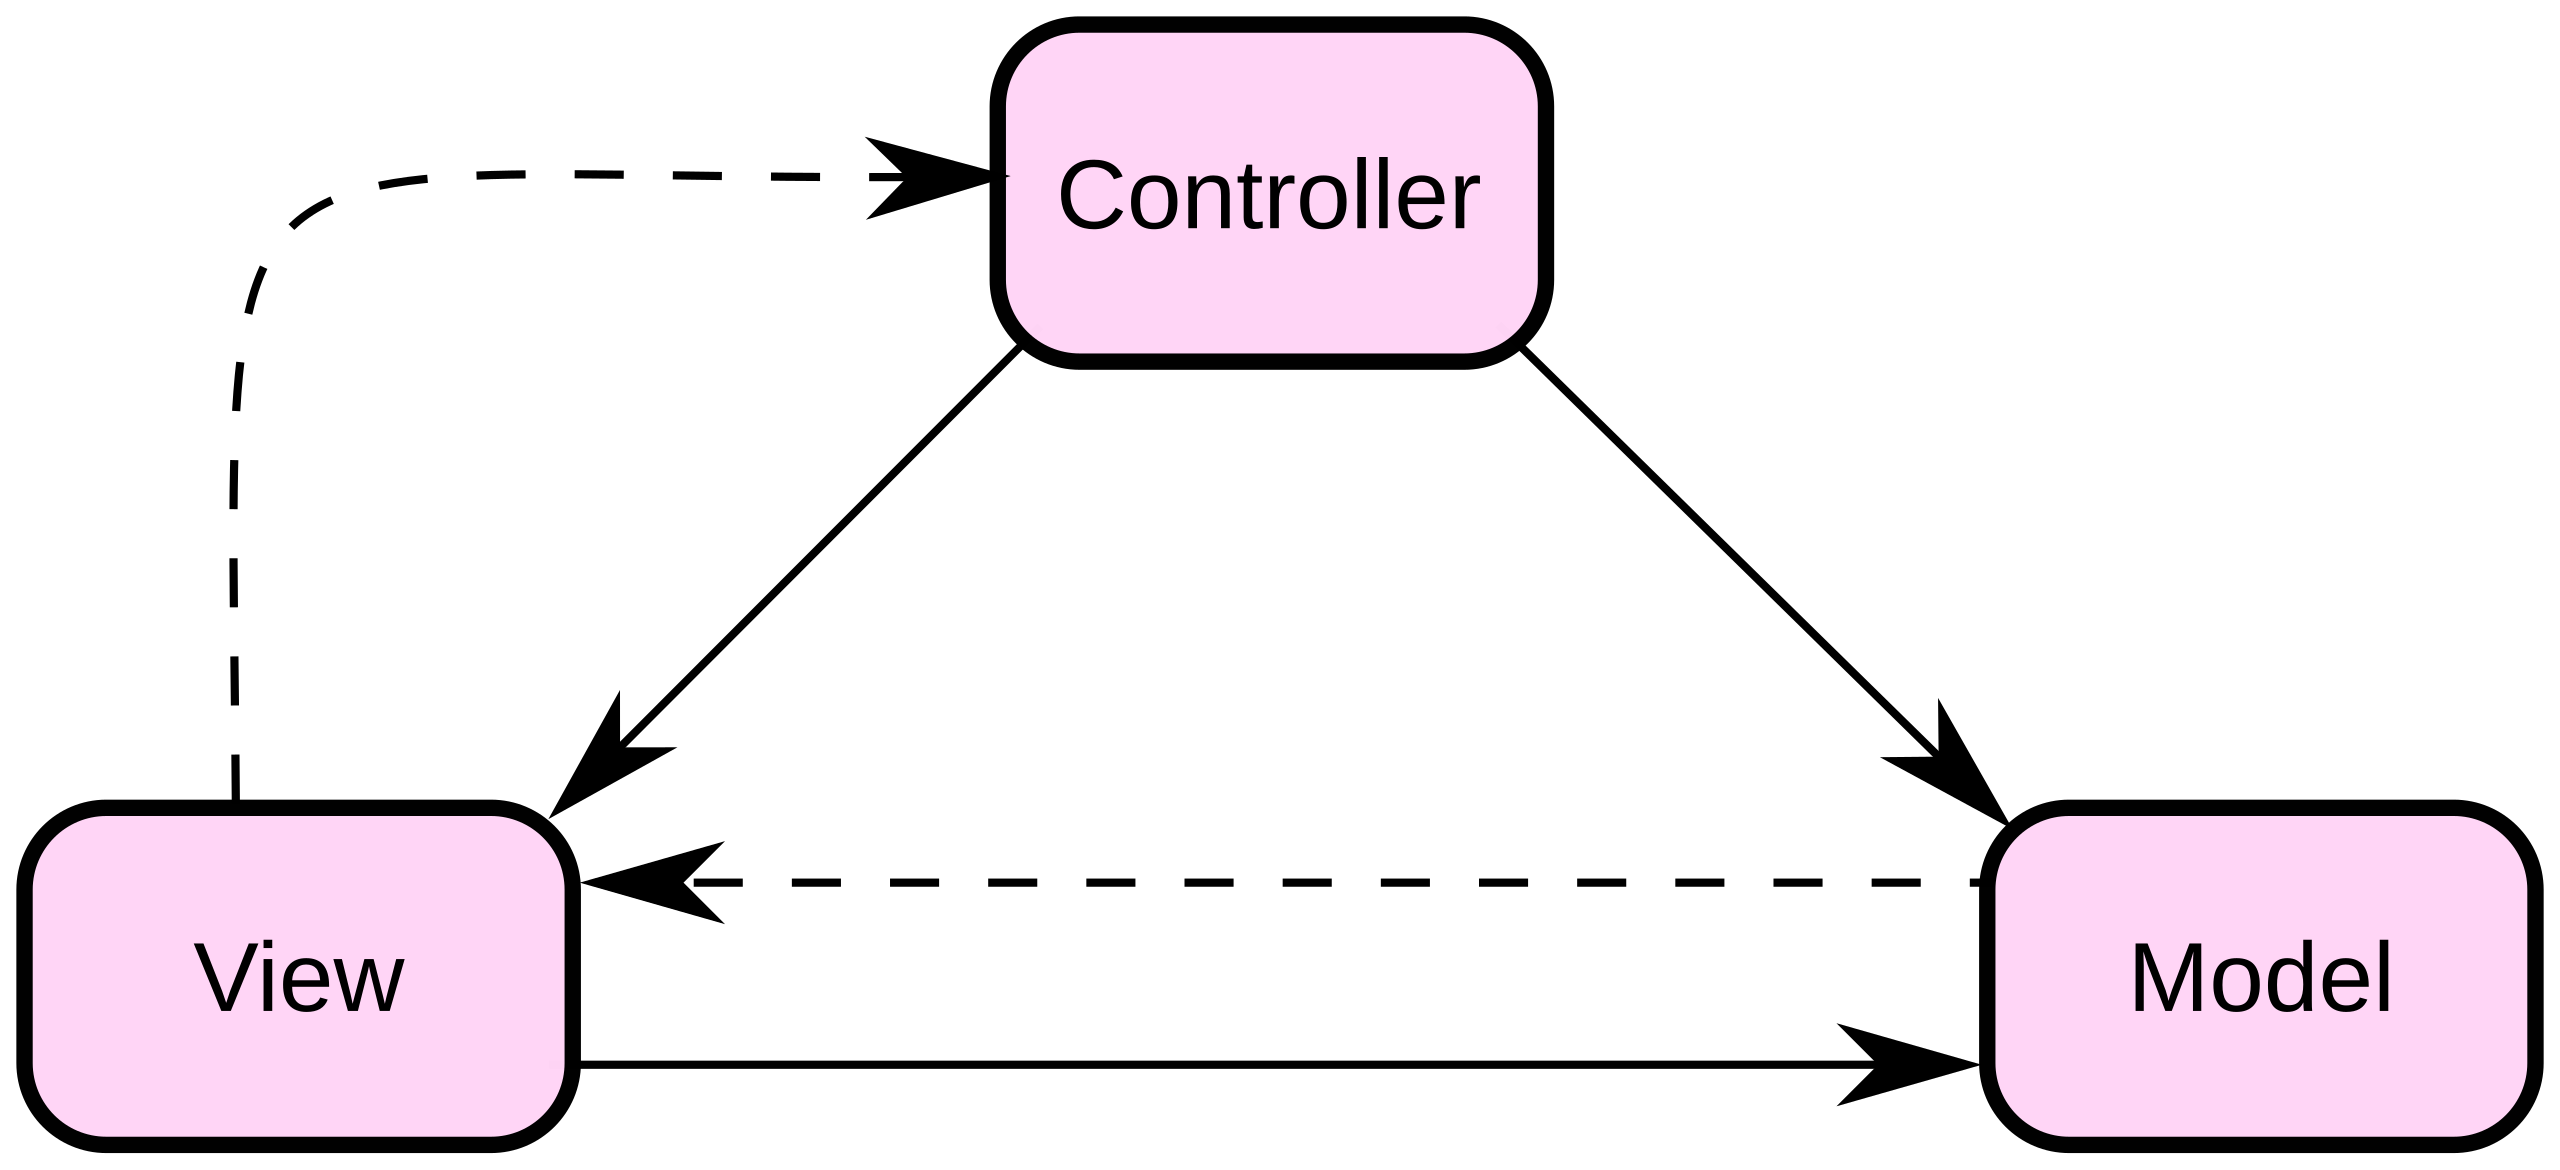
\includegraphics[width=0.8\textwidth]{MVC_struktur.png}
    \caption{Schematische Darstellung der MVC Struktur \cite{noauthor_model_2024}} 
    \label{fig:MVC_struktur}
\end{figure}

Im Rahmen dieser Studienarbeit gibt es keine externen Anforderungen an die Struktur. Daher wurde sich für eine vereinfachte \ac{MVC} Struktur entschieden (\autoref{fig:MVC_struktur}). Ziel dieser Struktur ist es die Software in drei Teile zu unterteilen.
Diese drei Teile sollen eigenständige Aufgaben übernehmen und so verhindern, dass das Programm zu einem monolithischen Codeblock wird.

Der Model-Teil ist für die Datenverarbeitung zuständig und enthält die Datenstrukturen sowie die Logik, die die Daten verarbeitet. Der View-Teil ist für die Darstellung der Daten verantwortlich und umfasst die Benutzeroberfläche sowie die Logik, die die Daten darstellt. Der Controller-Teil steuert die Daten und koordiniert die Kommunikation zwischen Model und View, indem er die entsprechende Logik enthält.

Die vereinfachte Version dieser Struktur kombiniert die Funktionalitäten von View und Controller in der API. (Siehe \autoref{fig:flask}) und trennt die Datenverarbeitung in einem eigenen Modul, dem Pycore Modul, welches die benötigten selbst entwickelten Bibliotheken zur Verfügung stellt. 

\begin{figure}[H]
    \centering
    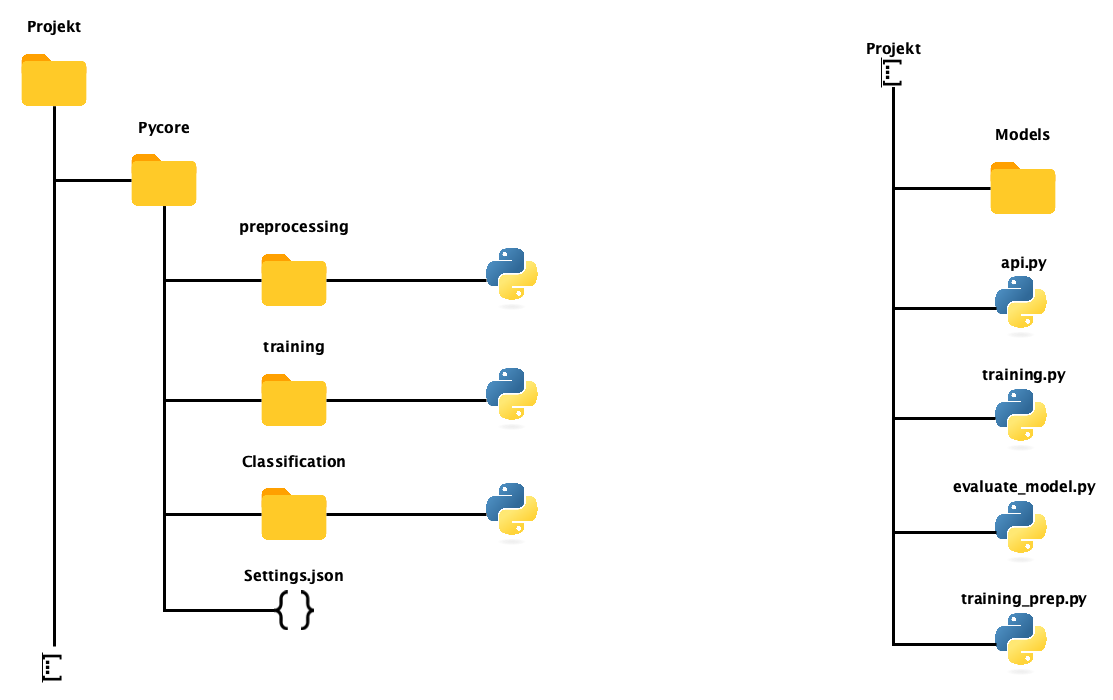
\includegraphics[width=0.8\textwidth]{Projektstruktur.png}
    \caption{Projektstruktur der Software im Dateiverzeichnis}
    \label{fig:Projektstruktur}
\end{figure}

Die in der Grafik \autoref{fig:Projektstruktur} dargestellte Dateistruktur repräsentiert ebenso die Struktur der Software. Die Funktionen werden in Bibliotheken im Pycore-Verzeichnis zusammengefasst. 
Sämtliche Daten werden in einem ausgegliederten Verzeichnis innerhalb des Projektverzeichnisses abgelegt. 

Im Projekthauptverzeichnis gibt es vier Python Skrpte, die ausgeführt werden können, um einzelne Teile der Software auszuführen.
\texttt{api.py} Wird ausgeführt, um die Weboberfläche zu starten.
\texttt{train.py} Wird ausgeführt, um das Modell zu trainieren.
\texttt{evaluate\_model.py} Wird ausgeführt, um das Modell zu evaluieren und die in \autoref{sec:confusionmatrix}. Beschriebenen Werte zu erhalten. 
\texttt{training\_prep.py} Kann ausgeführt werden um den Datensatz zu verarbeiten ohne das Modell zu trainieren.

Diese Skripte laden den jeweilig benötigten Programmteil und die benötigten Parameter aus dem Pycore Verzeichnis, führen die entsprechenden Funktionen aus und legen die Ergebnisse im Dateisystem ab.


\section{Konfiguration} \label{sec:konfiguration}

Aus der Aufgabenstellung (siehe \autoref{sec:problemstellung_und_ziel_dieser_arbeit}) lässt sich ein weiterer Teil des Softwarekonzepts, die Einstellbarkeit, ableiten.
Durch die Einstellbarkeit soll gewährleistet sein, dass die Software flexibel an die Anforderungen des Benutzers angepasst werden kann, ohne dass der Benutzer ein tiefes Verständnis der Software haben muss.

\begin{lstlisting}[style=json, label=lst:json_example, caption={Beispiel einer \ac{JSON}-Datei mit Parametern des mobilnet Modells}]
    {
        "filepaths": {
            "good": "Bilder/Good_Pictures",
            "bad": "Bilder/Bad_Pictures",
            "good_gray": "Bilder/Good_Grayscale",
            "bad_gray": "Bilder/Bad_Grayscale",
            "train": "Bilder/train",
            "test":"Bilder/test",
            "validate":"Bilder/validate",
            "new": "Bilder/new"
        }
    }
\end{lstlisting}

Ziel ist es das der Benutzer eine einzige Datei öffnet und dort alle Einstellungen vornehmen kann. 
Diese Datei soll im \ac{JSON}-Format vorliegen, da es ein weit verbreitetes Format ist und von vielen Programmiersprachen unterstützt wird \cite{gur_diskussion_2024}.

Die Struktur der \ac{JSON}-Datei ist in \autoref{lst:json_example} dargestellt und wird in Pyton mittels des \texttt{json} Moduls eingelesen. Ein Beispiel für das Einlesen der Datei ist in \autoref{lst:json_read} dargestellt.

Hier wird der Pfad zur Konfigurationsdatei festgelegt und die Datei wird eingelesen. Die Parameter werden dann an die erste Funktion übergeben, welche die Bilder in Graustufen umwandelt und in einem seperaten Verzeichnis ablegt (siehe \autoref{lst:json_read}). 

\begin{lstlisting}[style=python, label=lst:json_read, caption={Einlesen der \ac{JSON}-Datei}]
    import json

    config_path = "pycore/setings.json"
    cf = json.load(open(config_path, 'r'))

    # Uebergabe der Parameter an die Funktionen
    uic.folder_to_grayscale(cf["filepaths"]["good"],cf["filepaths"]["good_gray"])
    uic.folder_to_grayscale(cf["filepaths"]["bad"],cf["filepaths"]["bad_gray"])

\end{lstlisting}

Angenommen der Benutzer wünscht ein anderes Verzeichnis für die Bilder, so kann er dies in der \ac{JSON}-Datei ändern und die Software erneut ausführen, ohne zu wissen, wo die Funktion, welche den Datensatz generiert abliegt.

\section{Die Weboberfläche mittels Python Web API} \label{sec:weboberflaeche}